% Compilar con: pdflatex informe.tex  (también funciona con tectonic / Overleaf)
\documentclass[11pt,a4paper]{article}
\usepackage{iftex}
\ifPDFTeX
  \usepackage[utf8]{inputenc}
  \usepackage[T1]{fontenc}
  \usepackage{lmodern}
\else % XeLaTeX / LuaLaTeX / tectonic
  \usepackage{fontspec}
\fi
\usepackage[spanish,es-noshorthands,es-tabla]{babel}
\usepackage[margin=2.2cm]{geometry}
\usepackage{amsmath,amssymb}
\usepackage{graphicx}
\usepackage{booktabs}
\usepackage{tabularx}
\usepackage{array}
\usepackage{enumitem}
\usepackage[hidelinks]{hyperref}
\usepackage{xcolor}
\usepackage[most]{tcolorbox}

\setlist{nosep,leftmargin=1.4em}
\setlength{\parskip}{0.5em}
\setlength{\parindent}{0pt}
\newtcolorbox{respuesta}{colback=black!3,colframe=black!70,boxrule=0.8pt,arc=0pt,left=6pt,right=6pt,top=4pt,bottom=4pt}
\newcommand{\cin}[1]{#1_{\mathrm{in}}}
\newcommand{\cout}[1]{#1_{\mathrm{out}}}

\begin{document}

% ---------------------------------------------------------------- portada
\begin{titlepage}
\centering
{\large UNIVERSIDAD SAN FRANCISCO DE QUITO\\COLEGIO DE CIENCIAS E INGENIERÍAS\par}
\vspace{0.8cm}
{\large\bfseries CMP-4007 --- Algoritmos Avanzados\par}
\vspace{4cm}
{\LARGE\bfseries ¿Cuántos cables tienen que fallar?\par}
\vspace{0.4cm}
{\large Resiliencia de la red de cables submarinos\\con flujo máximo y corte mínimo\par}
\vspace{4cm}
{\large Julián León\\Adrián Torres\par}
\vspace{0.6cm}
{17 de noviembre de 2026\par}
\vfill
{\small Código: \url{https://github.com/jjjulianleon/mincutSCM}\\
Demo interactiva: \url{https://jjjulianleon.github.io/mincutSCM/}\par}
\end{titlepage}

% ---------------------------------------------------------------- declaración IA
\section*{Declaración de uso de inteligencia artificial}
En este trabajo usamos \textbf{Claude Code} (Anthropic), un asistente de IA que funciona como agente, para:
\begin{itemize}
  \item ubicar en los libros del curso las secciones que respaldan el modelo (CLRS, Kleinberg \& Tardos y Erickson);
  \item discutir las decisiones de modelado: qué es un vértice, cómo se representa un cable, qué cuenta como ruta, qué cables entran y qué es «Estados Unidos». Cada decisión se discutió con opciones y la aprobamos antes de implementarla;
  \item escribir el código en Python (descarga de datos, Edmonds--Karp y corte mínimo) y la demo interactiva;
  \item redactar este informe.
\end{itemize}
Todos los resultados numéricos provienen de ejecutar ese código sobre los datos de TeleGeography descargados el 17 de noviembre de 2026; ninguno fue escrito a mano ni generado como texto. El código incluye pruebas con los ejemplos de las presentaciones de clase (flujo máximo 5 y corte mínimo 12), y en cada país verifica que el número de cables del corte coincida con el valor del flujo.

\newpage
% ---------------------------------------------------------------- modelo
\section*{Planteamiento del modelo}
Los datos son el \emph{Submarine Cable Map} de TeleGeography (CC BY-SA 4.0). Para cada cable dan su nombre, si está planeado (\texttt{is\_planned}) y la lista de estaciones donde toca tierra, con el país de cada una. \textbf{No} dan la capacidad del cable ni el orden de sus tramos.

\subsection*{La red}
\begin{tabularx}{\textwidth}{@{}l X@{}}
\toprule
Decisión & Elección y motivo\\
\midrule
Vértices & Un vértice por país. Supuesto: las estaciones de un mismo país están conectadas por tierra. Las tres preguntas hablan de países.\\
Cables & Cada cable $c$ es un vértice partido en $\cin{c}\to\cout{c}$ con capacidad~1 (capacidad en vértices, Erickson §11.2). Para cada país $p$ que toca, se agregan $p\to\cin{c}$ y $\cout{c}\to p$ con capacidad~$\infty$.\\
Rutas & Una ruta puede pasar por otros países, cambiando de cable dentro de cada país.\\
Cables incluidos & Solo los cables en servicio (\texttt{is\_planned = false}) y que tocan al menos dos países. Un cable doméstico no puede formar parte de una ruta entre países. Como comparación, se calcula también el escenario que incluye los planeados.\\
Estados Unidos & Todo lo que el dataset etiqueta \texttt{United States} (incluye Puerto Rico).\\
\bottomrule
\end{tabularx}

\textbf{Por qué un cable es un vértice y no una arista.} La pregunta cuenta cables que fallan, y un cable que toca varios países falla una sola vez. Si un cable que toca Ecuador, Panamá y EE.\,UU. se modelara como tres aristas de capacidad~1 (una por par de países), todo corte entre Ecuador y EE.\,UU. tendría que cortar dos de ellas, y el corte valdría~2 aunque basta que falle un cable. Con el cable como vértice, ese corte vale~1. Las aristas país--cable valen~$\infty$ para que el corte nunca «rompa la llegada» de un cable a un país: solo puede romper el cable completo.

\subsection*{Qué mide $n$}
Sea $P$ el número de países con cables internacionales y $K$ el número de cables internacionales en servicio. Sea $k_c$ el número de países que toca el cable~$c$. La red tiene
\[
|V| = P + 2K, \qquad |E| = K + 2\sum_c k_c .
\]
Con los datos del 17 de noviembre de 2026: $P=184$, $K=330$, $\mathbf{|V|=844}$ y $\mathbf{|E|=2542}$. El tamaño de la entrada, $n$, es el par $(|V|,|E|)$.

\subsection*{Algoritmo}
Para cada país $p$ se toma $s=p$ y $t=$ Estados Unidos, y se corre \textbf{Edmonds--Karp}: Ford--Fulkerson que elige siempre el camino aumentante con menos aristas mediante BFS en la red residual $G_f$ (presentación \emph{Max-flow}, diap.~5). Después se hace \textbf{una BFS más} en $G_f$. El conjunto $S$ de vértices alcanzables desde $s$ define el corte $(S,T)$, y los cables cuya arista $\cin{c}\to\cout{c}$ cruza de $S$ a $T$ son los que hay que romper (presentación \emph{Min-cut}, diap.~7).

\textbf{Certificado.} Como todas las capacidades finitas son~1, el flujo máximo se descompone en $|f|$ rutas que no comparten cable, y por el teorema de flujo máximo y corte mínimo $|f| = c(S,T)$ (en este caso particular es el teorema de Menger, Kleinberg \& Tardos §7.6, (7.45)). Las rutas prueban que con menos de $|f|$ fallas no alcanza, porque cada falla rompe a lo sumo una ruta. El corte prueba que $|f|$ fallas sí alcanzan. El programa comprueba en cada país que el número de cables del corte sea igual a $|f|$.

\subsection*{Complejidad}
Sea $g(p)$ el número de cables internacionales que tocan $p$ (la «medida ingenua»).
\begin{itemize}
  \item \textbf{Una corrida.} El corte $S_0=\{p\}\cup\{\cin{c} : c \text{ toca } p\}$ tiene capacidad exactamente $g(p)$, porque las únicas aristas que salen de $S_0$ son las $\cin{c}\to\cout{c}$ de esos cables. Por dualidad débil (\emph{Min-cut}, diap.~6), $|f^*|\le g(p)$. Con capacidades enteras, cada aumento sube $|f|$ en al menos~1 y cuesta $O(|V|+|E|)$ (una BFS más la actualización del camino). Por eso Edmonds--Karp hace a lo sumo $g(p)$ aumentos, y una corrida cuesta $O(g(p)\cdot|E|)$ (es la cota $O(|E|\cdot|f^*|)$ de \emph{Max-flow}, diap.~6). La BFS final cuesta $O(|V|+|E|)$.
  \item \textbf{Todos los países (literal~3).} $\sum_p g(p) = \sum_c k_c \le |E|/2$, así que el total es $O(|E|^2)$.
\end{itemize}
Se escribe $O$ y no $\Theta$ porque son cotas superiores: no se demostró que se alcancen. En la práctica, los 183 países se calculan en 1{,}4\,s.

{\small La implementación ordena los vecinos en cada BFS para que los resultados sean reproducibles. Eso agrega un factor logarítmico que el análisis anterior no incluye.\par}

\newpage
% ---------------------------------------------------------------- literal 1
\section*{Literal 1 --- Ecuador}
\begin{respuesta}
\textbf{Respuesta:} tienen que fallar, como mínimo, \textbf{4 cables}: Pacific Caribbean Cable System (PCCS), PanAm South, South America-1 (SAm-1) y South Pacific Cable System (SPCS)/Mistral.
\end{respuesta}

\subsection*{Por qué con 3 no alcanza: 4 rutas que no comparten cable}
\begin{tabularx}{\textwidth}{@{}c X l@{}}
\toprule
\# & Ruta & Estación en Ecuador\\
\midrule
1 & Ecuador $\to$ [PCCS] $\to$ EE.\,UU. & Manta\\
2 & Ecuador $\to$ [SAm-1] $\to$ EE.\,UU. & Punta Carnero\\
3 & Ecuador $\to$ [PanAm South] $\to$ Panamá $\to$ [ARCOS] $\to$ EE.\,UU. & Punta Carnero\\
4 & Ecuador $\to$ [SPCS/Mistral] $\to$ Chile $\to$ [Curie] $\to$ EE.\,UU. & Salinas\\
\bottomrule
\end{tabularx}

Ningún cable aparece en dos rutas. Cada falla rompe a lo sumo una, así que con 3 fallas siempre sobrevive al menos una ruta.

\subsection*{Por qué con 4 sí alcanza: el corte}
Después del cuarto aumento ya no hay camino de Ecuador a EE.\,UU. en $G_f$. La BFS final alcanza solo a Ecuador y a la entrada de sus cuatro cables, porque los cuatro están llenos. Esos cuatro cables forman el corte, y su capacidad es $4=|f|$.

El programa también calcula el corte mínimo «más cercano a $t$» (los vértices que llegan a EE.\,UU. en $G_f$), y coincide con el anterior.

\subsection*{Lectura}
Ecuador tiene 4 cables internacionales en servicio y hay que romper 4. Cada cable aporta una ruta independiente, así que \textbf{no hay un cuello de botella escondido}: la medida ingenua y el min-cut coinciden. Si se incluye CSN-1 (Ancón), que en los datos figura como planeado para 2026, el resultado sube a~5.

Ojo: SAm-1 y PanAm South llegan a la misma estación, Punta Carnero. El modelo trata sus fallas como independientes, pero un mismo evento local podría afectar a ambos (ver literal~3).

\begin{center}
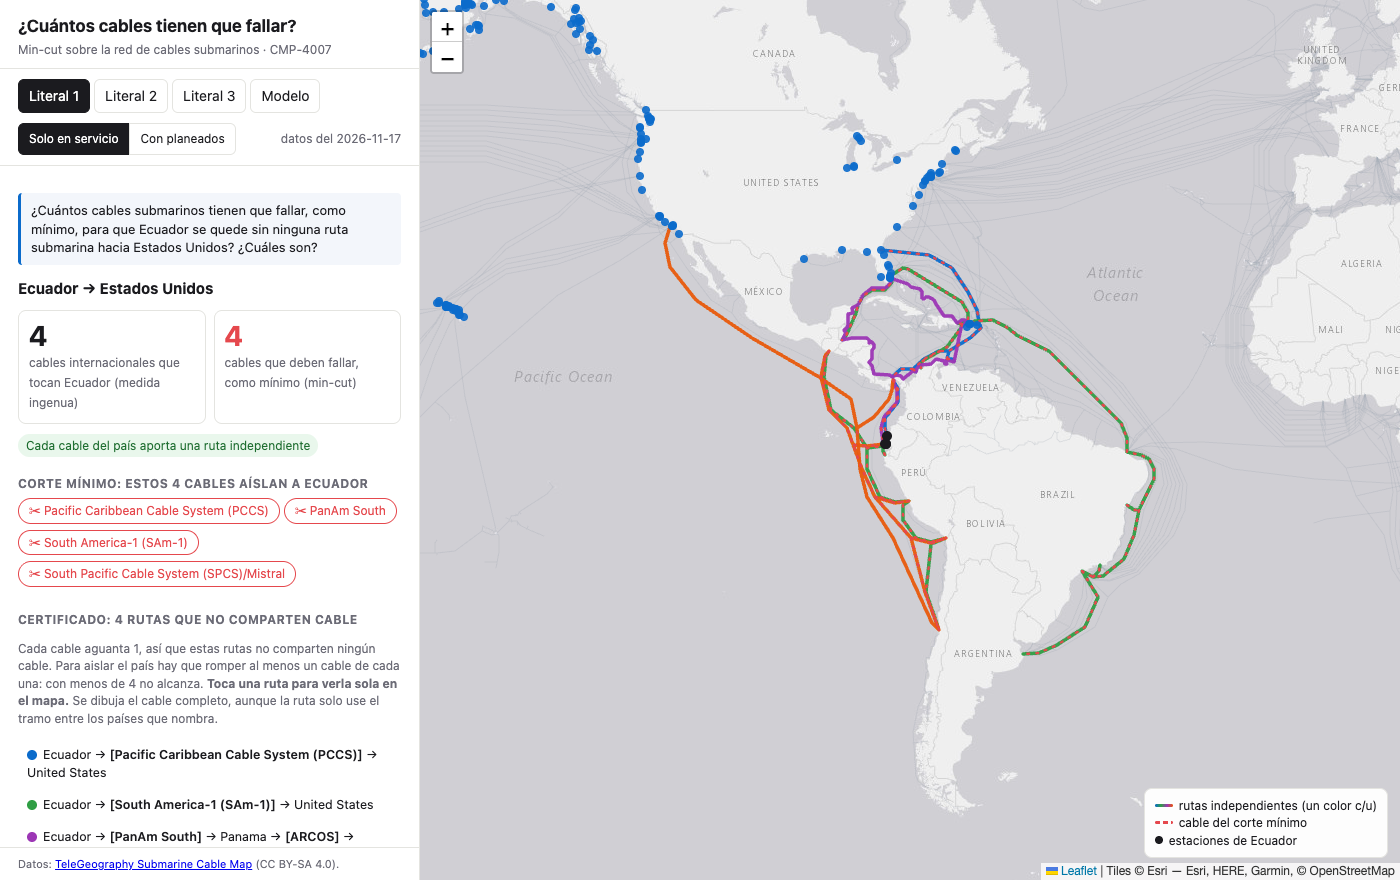
\includegraphics[width=0.62\textwidth]{demo_literal1.png}\\[2pt]
{\small Demo interactiva, Literal~1. Cada ruta se dibuja en su color y los cables del corte llevan un trazo rojo punteado.}
\end{center}

\newpage
% ---------------------------------------------------------------- literal 2
\section*{Literal 2 --- Ranking}
\begin{respuesta}
\textbf{Respuesta} (del más al menos resiliente): Brasil, Colombia, Panamá, Argentina, Chile, Ecuador, México, Uruguay, Venezuela y Perú.
\end{respuesta}

\begin{center}
\begin{tabular}{@{}r l r r@{}}
\toprule
\# & País & Min-cut (cables que deben fallar) & Cables internacionales\\
\midrule
1 & Brasil & 11 & 13\\
2 & Colombia & 7 & 7\\
3 & Panamá & 6 & 6\\
4 & Argentina & 5 & 7\\
5 & Chile & 4 & 4\\
6 & Ecuador & 4 & 4\\
7 & México & 4 & 4\\
8 & Uruguay & 4 & 4\\
9 & Venezuela & 4 & 4\\
10 & Perú & 3 & 3\\
\bottomrule
\end{tabular}
\end{center}

\textbf{Criterio.} Se ordena por min-cut, de mayor a menor. Si hay empate, gana el que tiene más cables internacionales. Si sigue el empate, se ordena por nombre. Chile, Ecuador, México, Uruguay y Venezuela empatan en ambas medidas (4 y 4): son igual de resilientes según esta medida, y su orden entre ellos es solo alfabético.

\textbf{Lo que el min-cut ve y el conteo no.}
\begin{itemize}
  \item \textbf{Argentina} tiene 7 cables, pero bastan 5 fallas: Firmina, Malbec, SAm-1, SAC y Tannat. Los otros dos, Bicentenario y Unisur, solo la unen con Uruguay. Como Uruguay queda del lado de Argentina en el corte, toda ruta de Uruguay a EE.\,UU. usa alguno de esos 5 cables.
  \item \textbf{Brasil} pasa de 13 a 11 por la misma razón: Malbec y Tannat lo unen con Argentina y Uruguay, que no aportan rutas nuevas.
\end{itemize}

\textbf{México} tiene frontera terrestre con EE.\,UU., pero la pregunta es por rutas \emph{submarinas}, así que esa conexión no entra en el modelo.

\newpage
% ---------------------------------------------------------------- literal 3
\section*{Literal 3 --- El más resiliente del mundo}
\begin{respuesta}
\textbf{Respuesta:} según esta medida, el país más resiliente es \textbf{Singapur}: tienen que fallar al menos 27 de sus 34 cables internacionales para aislarlo de Estados Unidos.
\end{respuesta}

\begin{center}
\begin{tabular}{@{}r l r r @{\hspace{1.5em}} r l r r@{}}
\toprule
\# & País & Min-cut & Cables & \# & País & Min-cut & Cables\\
\midrule
1 & Singapur & 27 & 34 & 6 & Malasia & 20 & 20\\
2 & Francia & 24 & 24 & 7 & Egipto & 16 & 17\\
3 & Reino Unido & 23 & 51 & 8 & Emiratos Árabes Unidos & 16 & 17\\
4 & Japón & 23 & 24 & 9 & China & 16 & 16\\
5 & Indonesia & 23 & 23 & 10 & India & 16 & 16\\
\bottomrule
\end{tabular}
\end{center}

Se calculó lo mismo para los 183 países con cables internacionales; EE.\,UU. no participa porque no se puede aislar de sí mismo. El caso del \textbf{Reino Unido} es el que mejor muestra la idea del problema: tiene 51 cables, pero muchos van a Irlanda, la Isla de Man, Guernsey o Países Bajos, y desde ahí siguen por los mismos cables trasatlánticos. Basta romper 23.

\subsection*{¿Le creemos?}
\textbf{Solo en parte.} El número es correcto \emph{para el modelo}: está certificado por 27 rutas disjuntas y un corte de 27 cables. Pero el modelo hace supuestos que lo alejan de la realidad:
\begin{itemize}
  \item \textbf{Tránsito terrestre gratis e ilimitado.} El modelo supone que dentro de cada país se puede pasar de un cable a cualquier otro. Por eso aparecen rutas como Francia $\to$ Jordania $\to$ Malasia $\to\cdots\to$ EE.\,UU., de hasta 11 saltos. Esas rutas existen físicamente, pero dependen de redes terrestres, acuerdos entre operadores y la situación política de cada país. Singapur se beneficia especialmente de esto, porque muchas de sus rutas siguen por Malasia, Indonesia y otros países vecinos.
  \item \textbf{Fallas independientes.} El modelo cuenta cada falla por separado, pero varios cables comparten estación o corredor. De los 34 cables de Singapur, 14 llegan a Tuas y 10 a Changi North. Un ancla o un terremoto en uno de esos puntos rompe varios a la vez. Lo mismo pasa a menor escala con Punta Carnero en Ecuador.
  \item \textbf{Todos los cables valen lo mismo.} El modelo no mira la capacidad, así que un cable de 1999 cuenta igual que uno moderno con cien veces más ancho de banda. «Seguir conectado» no es lo mismo que «seguir funcionando con normalidad».
  \item \textbf{La medida depende del destino.} Medimos el aislamiento respecto de EE.\,UU. Si el destino fuera otro país, el ranking podría cambiar. Lo que el modelo responde es «el país más difícil de desconectar de EE.\,UU.», no «el más resiliente en general».
  \item \textbf{Datos incompletos.} El dataset no da el orden de los tramos, así que se supone que un cable falla entero, cuando en realidad un corte suele afectar un solo tramo. Además es una foto del 17 de noviembre de 2026: los cables planeados pueden cambiar el resultado. En Ecuador, por ejemplo, el corte sube de 4 a 5 con CSN-1.
\end{itemize}
En conclusión, el modelo sirve para \textbf{comparar} países y para encontrar cuellos de botella escondidos, como en el Reino Unido o Argentina. Pero el valor 27 de Singapur no debe leerse como «hacen falta 27 accidentes»: por las fallas correlacionadas y el tránsito por terceros países, la resiliencia real es menor.

\newpage
% ---------------------------------------------------------------- fuentes
\section*{Fuentes y colaboración}
\begin{itemize}
  \item \textbf{Datos:} TeleGeography, \emph{Submarine Cable Map}, \url{https://www.submarinecablemap.com} (CC BY-SA 4.0), descargados el 17 de noviembre de 2026.
  \item \textbf{Material de clase:} presentaciones \emph{Max-flow} y \emph{Min-cut} (CMP-4007).
  \item \textbf{Libros:} Erickson, \emph{Algorithms} (2019), cap.~10 (historia de Harris y Ross) y §11.1--11.2 (caminos disjuntos y capacidades en vértices, pp.~353--354); Kleinberg \& Tardos, \emph{Algorithm Design}, §7.6 (teorema de Menger, (7.45)); Cormen et al., \emph{Introduction to Algorithms}, 4.\textsuperscript{a} ed., §24.1 (aristas antiparalelas y varias fuentes, pp.~673--674).
  \item \textbf{Integrantes:} Julián León y Adrián Torres. No colaboramos con otros compañeros.
  \item \textbf{Inteligencia artificial:} Claude Code (Anthropic), un agente de IA. Lo usamos para buscar referencias, discutir el modelo, escribir el código y la demo, y redactar el informe (detalle en la declaración inicial). Verificamos por nuestra cuenta: que las pruebas reproducen los ejemplos de las presentaciones (flujo 5 y corte 12), que el modelo cuenta 1 en el ejemplo de un cable con tres países, y las rutas y el corte de Ecuador sobre el mapa.
  \item \textbf{Código y demo:} \url{https://github.com/jjjulianleon/mincutSCM}.
\end{itemize}

\end{document}
